\section{Implementierung des Constraint-Systems}\label{section:Implementierung des Constraint-Systems}

Das Constraint-System baut, wie in der Konzeptionalisierung aufgezeigt, auf den Ergebnissen der vorherigen Forschungsarbeiten auf.

Als Basis der Codebasis wird das JavaScript Build-System \textit{Vite} genutzt \parencite{voidzeroinc.Vite2025}. Das System automatisiert den für moderne Webanwendungen nötigen Übersetzungs- und Optimierungsprozess, bei welchem der Quelltext in TypeScript in eine für Browser interpretierbare Ausgabe umgewandelt wird. Vite löst hierfür Modulabhängigkeiten auf und bündelt statische Ressourcen, wodurch ein lauffähiges Artefakt entsteht.

Über den reinen Transpilationsschritt hinaus führt Vite in einem Produktionsbuild zusätzliche Optimierungen – etwa Code-Splitting, Tree-Shaking und Minifizierung – durch, um Ladezeiten und Bandbreitenbedarf zu minimieren.

\medskip

Wie in im Kapitel \ref{section:Technische Grundlagen} [S. \pageref{section:Technische Grundlagen}] zu technischen Grundlagen bereits aufgearbeitet, wird als Basis für die Darstellung React, react-three-fiber sowie die Erweiterung @react-three/xr genutzt.

Der Code für React-Anwendungen geschieht durch einen funktionalen Codestil, der Rest des Validierungssystem soll jedoch über eine objektorientierte Architektur umgesetzt werden.

\subsection{Aufbau des Codes}

Die Codebasis wurde in drei Haupteinheiten geteilt: Der Application Layer stellt den Kern des Validierungssystem und ist für das Parsing und Auswerten von Validierungen zuständig. Der Infrastructure Layer stellt Hilfssysteme für die Auswertung, darunter etwa zur Segmentierung der Umgebung. Zuletzt ist der Presentation Layer für die Darstellung der 3D Objekte und Validierungsergebnisse über React-Three-Fiber zuständig.

In der ersten Iteration wurde die Kommunikation zwischen Einheiten der Application und Infrastructure zunächst über ein \quoted{God Object} umgesetzt. Um dieses Anti-Pattern aufzulösen wurde diese Abhängigkeit durch die Nutzung von Dependency Injection mittels der TypeScript Bibliothek \textmono{tsyringe} umgesetzt - hierdurch werden alle Abhängigkeiten über einen einheitlichen IoC-Container aufgelöst werden. Zusätzlich können durch den Container Referenzen auf Interfaces oder abstrakte Klassen durch die konkret benötigten Implementierungen umgewandelt werden.

\subsubsection{Kernsystem: Application Layer}

\begin{figure}[h]
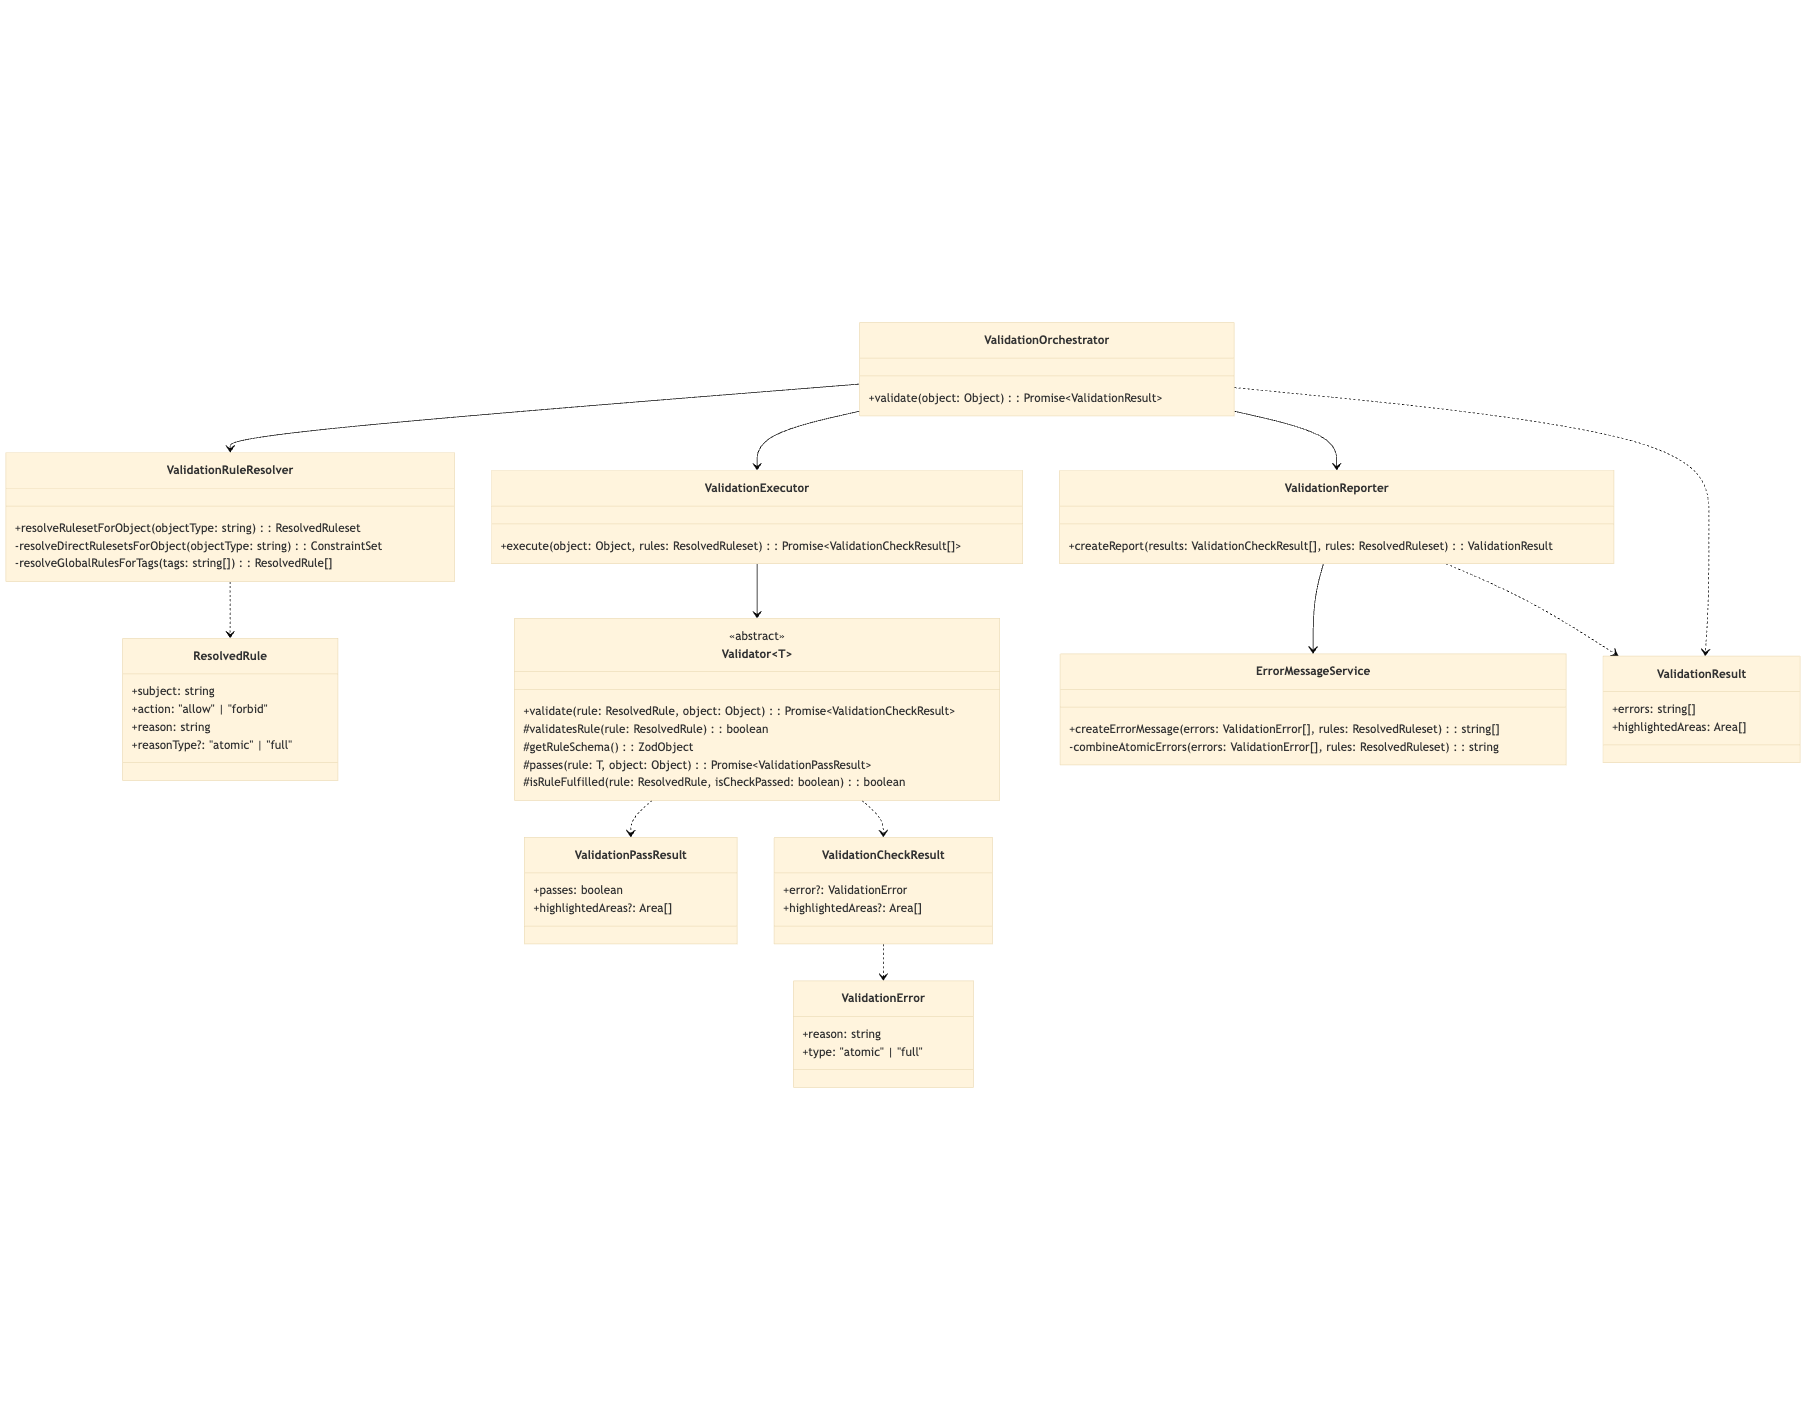
\includegraphics[width=1\textwidth]{abb/uml core system.png}
\centering
\caption{Klassendiagramm: Application Layer}
\label{fig:uml core system}
\end{figure}

Abbildung \ref{fig:uml core system} zeigt ein UML Klassendiagramm über den Aufbau des Kernsystems. Das oberste Objekt des Diagramms ist die Klasse \textmono{ValidationOrchestrator}, welche die Deligierung der Aufgaben an die einzelnen Subklassen unternimmt und für den Presentation Layer eine einheitliche API bereitstellt. Hierfür existiert die vorher konzeptionierte Funktion \textmono{validate(object: Object): Promise<ValidationResult>} zur Validierung.

Wie zuvor aufgezeigt erfolgt die Auflösung der Verbindungen zu den Subklassen über den Dependency Injection IoC-Container, um die einzelnen Aufgaben weiterzugeben.

Zur zentralen Verwaltung aller Objekte wurde eine Klasse \textmono{Object} umgesetzt. Diese Klasse enthält alle Informationen zum Objekttyp, Position, Skalierung, Rotation sowie einer Objekt ID zur eindeutigen Identifizierung einzelner Objekte im System. Zusätzlich setzt die Klasse das Observer Pattern durch die Implementierung eines \textmono{EventEmitters} um, wodurch alle Komponenten des Systems bei Veränderungen informiert werden.

\medskip

Zunächst ruft der Delegator daraufhin die Klasse \textmono{ValidationRuleResolver} mit der Funktion \textmono{resolveRulesetForObject} auf. Diese Klasse lädt alle Constraint-Rulset Dateien, um die objektspezifischen Regeln über die interne Methode \textmono{resolveDirectRulesetsForObject} sowie global anwendbaren Regeln über die interne Methode \textmono{resolveGlobalRulesForTags} aufzulösen. Alle anwendbaren Regeln werden schließlich zu einem \textmono{ResolvedRuleset} verbunden, welches von späteren Einheiten ausgeführt werden kann.

Der \textmono{ValidationOrchestrator} ruft daraufhin die Methode \textmono{execute(object: Object, rules: ResolvedRuleset)} des \textmono{ValidationExecutor} auf. Innerhalb dieser Methode werden die benötigten Validatoren erstellt und ausgeführt.

\medskip

Die tatsächliche Ausführung der Logik erfolgt über Validatoren, welche auf der abtrakten Klasse \textmono{Validator<RuleType>} aufbauen. Die abstrakte Klasse implementiert bereits einige Hilfsmethoden, um die Zuständigkeit für einzelne Regeln zu prüfen, das Schema der Regeln zu validieren sowie die Art der Regeln (\textmono{forbid} oder \textmono{allow-only}) auszuwerten. Die konkreten Implementierungen werden später genauer besprochen, diese müssen jedoch nur noch die Methode \textmono{passes} sowie konkrete Regel-Validierungen implementieren, um einen positiv-Test auf den Constraint durchzuführen.

Für die Erstellung der Validatoren wird das Factory Pattern angwendet, bei welchem die Factory-Funktion \textmono{createValidators} Instanzen aller Validatoren über den IoC-Container auflöst.

\medskip

Durch die einzelnen Validatoren sowie den \textmono{ValidationExecutor} werden schließlich ein Array an \textmono{ValidationCheckResult} zurückgemeldet, welche Informationen über den Fehlerstatus sowie betroffene Bereiche der Szene liefern.

Diese Information wird schließlich vom \textmono{ValidationOrchestrator} an die Subklasse \textmono{ValidationReporter} deligiert, welcher die einzelnen Fehler in zusammenhängende Fehlermeldungen zusammenfasst und über den \textmono{ErrorMessageService} formatiert.

\medskip

Ein zentraler Aspekt des Containt-Syntax sind \quoted{atomare Fehlermeldungen}, welche modular zu einem zusammenhängenden Satz kombiniert werden können. Die atomaten Fehler müssen hierbei im Format \quoted{Das Objekt muss [Fehlermeldung], damit [Grund]} formatiert werden, z.B. \quoted{1 Meter von einer Straße entfernt liegen, damit die Gefahr bei Unfällen minimiert wird} und \quoted{vollständig auf Gras platziert werden, damit es keine Fußgänger behindert}. Über den \textmono{ErrorMessageService} können diese einzelnen atomaren Fehler schließlich zu einer vollständigen Information zusammengefügt werden, z.B. \quoted{Die Sitzbank muss \textit{1 Meter von einer Straße entfernt liegen, damit die Gefahr bei Unfällen minimiert wird} und \textit{vollständig auf Gras platziert werden, damit es keine Fußgänger behindert}}.

Die vollständigen, kombinierten Fehlermeldungen werden schließlich zurück an den Presentation Layer gemeldet, damit diese dort dargestellt werden können.

\medskip

\begin{figure}[h]
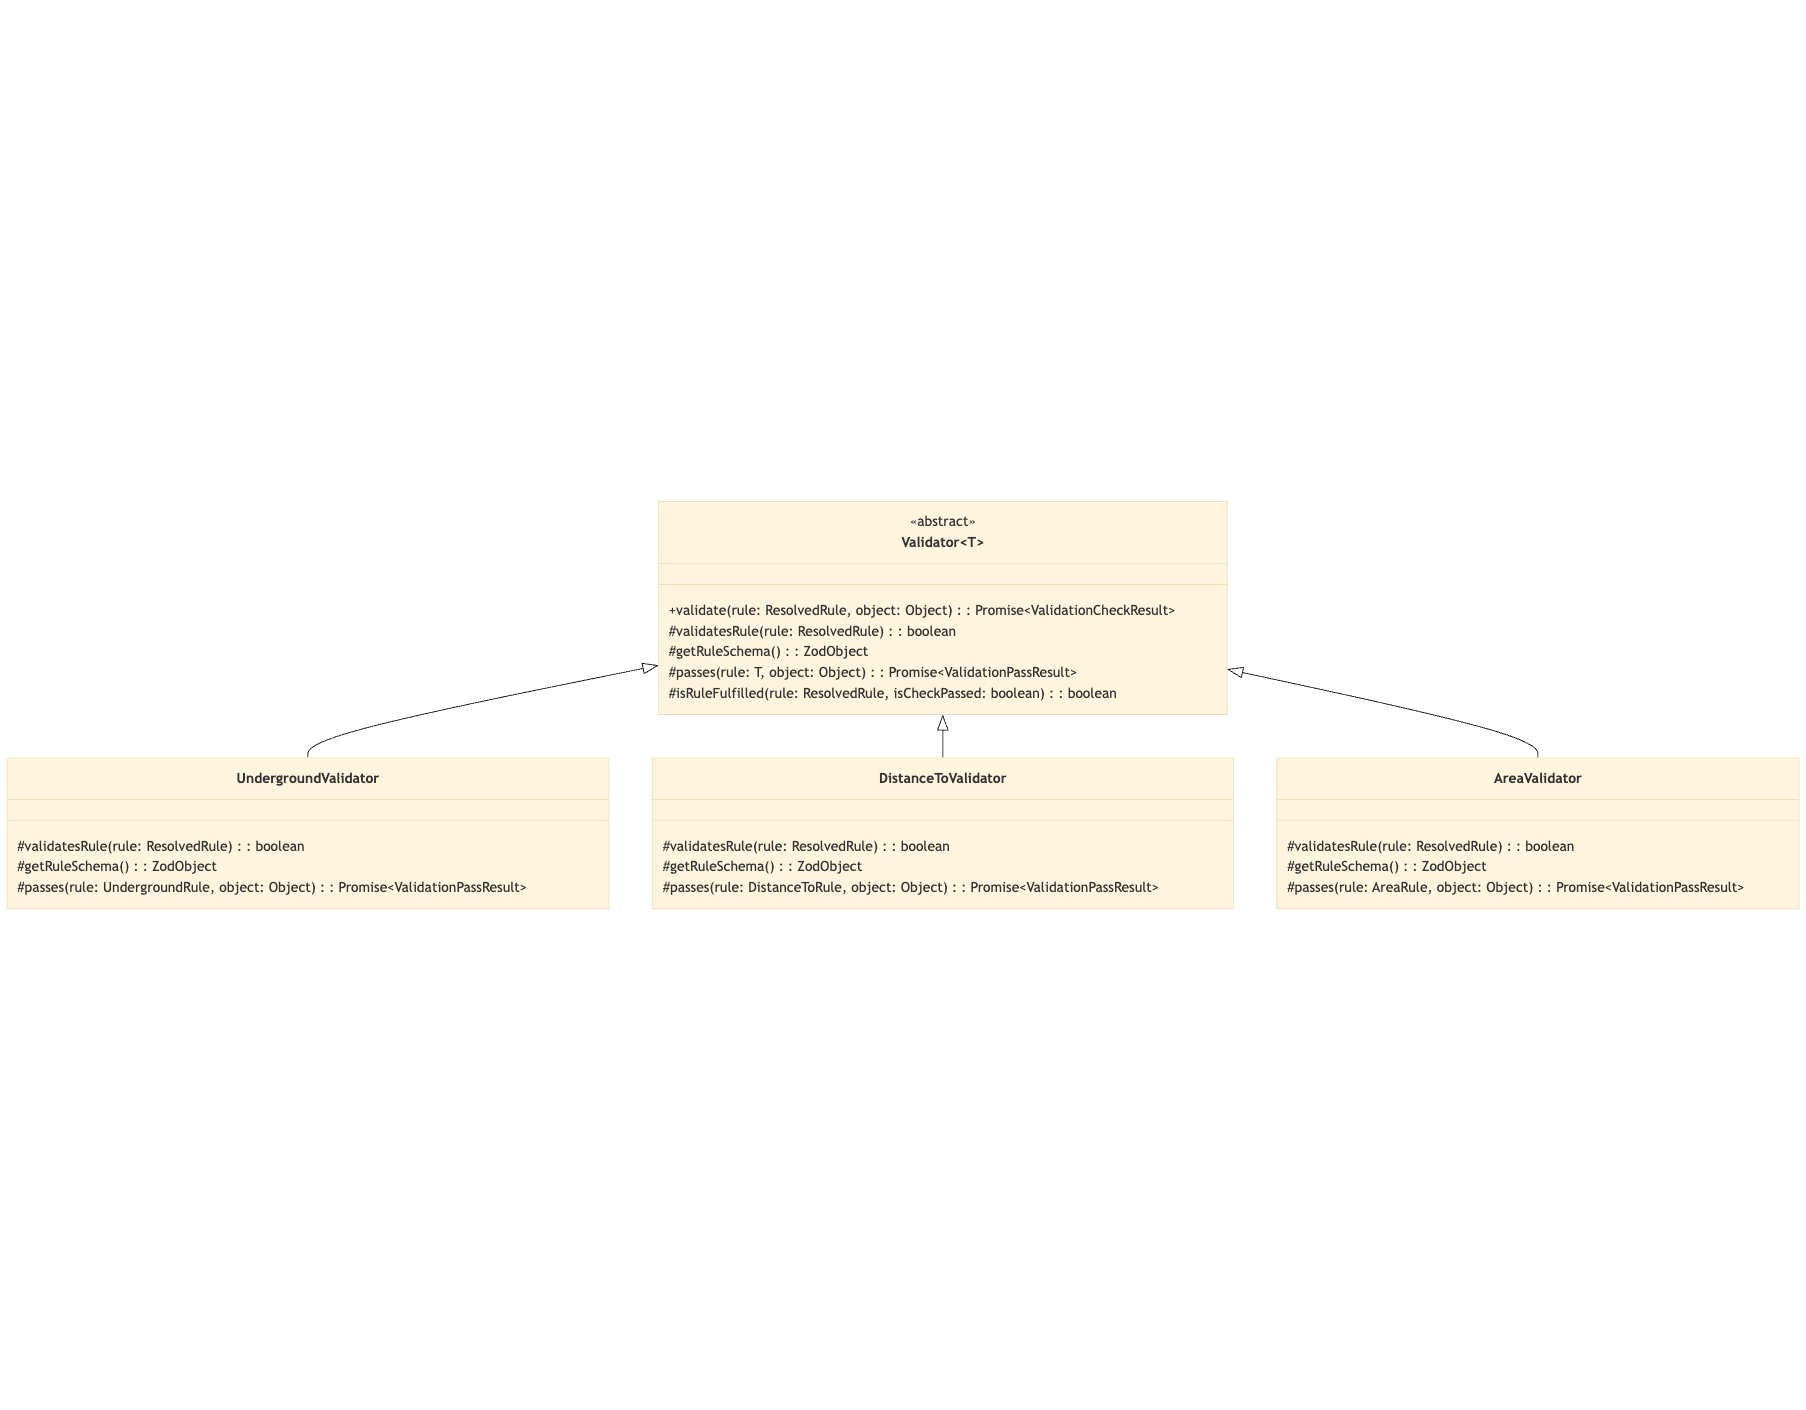
\includegraphics[width=1\textwidth]{abb/uml validators.png}
\centering
\caption{Klassendiagramm: Validatoren}
\label{fig:uml validators}
\end{figure}

Abbildung \ref{fig:uml validators} stellt ein weiteres UML Klassendiagramm zu einem Ausschnintt der konkreten Validatoren dar. Zentral sind hierbei vor allem der \textmono{UndergroundValidator} zur Validierung des Untergrunds, auf welchem das Objekt steht, \textmono{DistanceToValidator} zur Validierung der Abstands zu bestimmten Objektarten, sowie \textmono{AreaValidator} zur Validierung, ob sich das Objekt in einem bestimmten GeoJSON-Bereich befindet.

Für das System wird hierfür das Strategy Pattern implementiert, bei welchem die einzelnen Klassen die abstrakte Basisklasse erweitern, um geteilte Logik zu vererben, und erweitern diese mit konkreten Implementierungen der eigenen Validierung.

\subsubsection{Service-System: Infrastructure Layer}

Der Infrastructure Layer stellt diverse geteilte Services zur Verfügung, welche in den Validierungen gebraucht werden.

\begin{figure}[h]
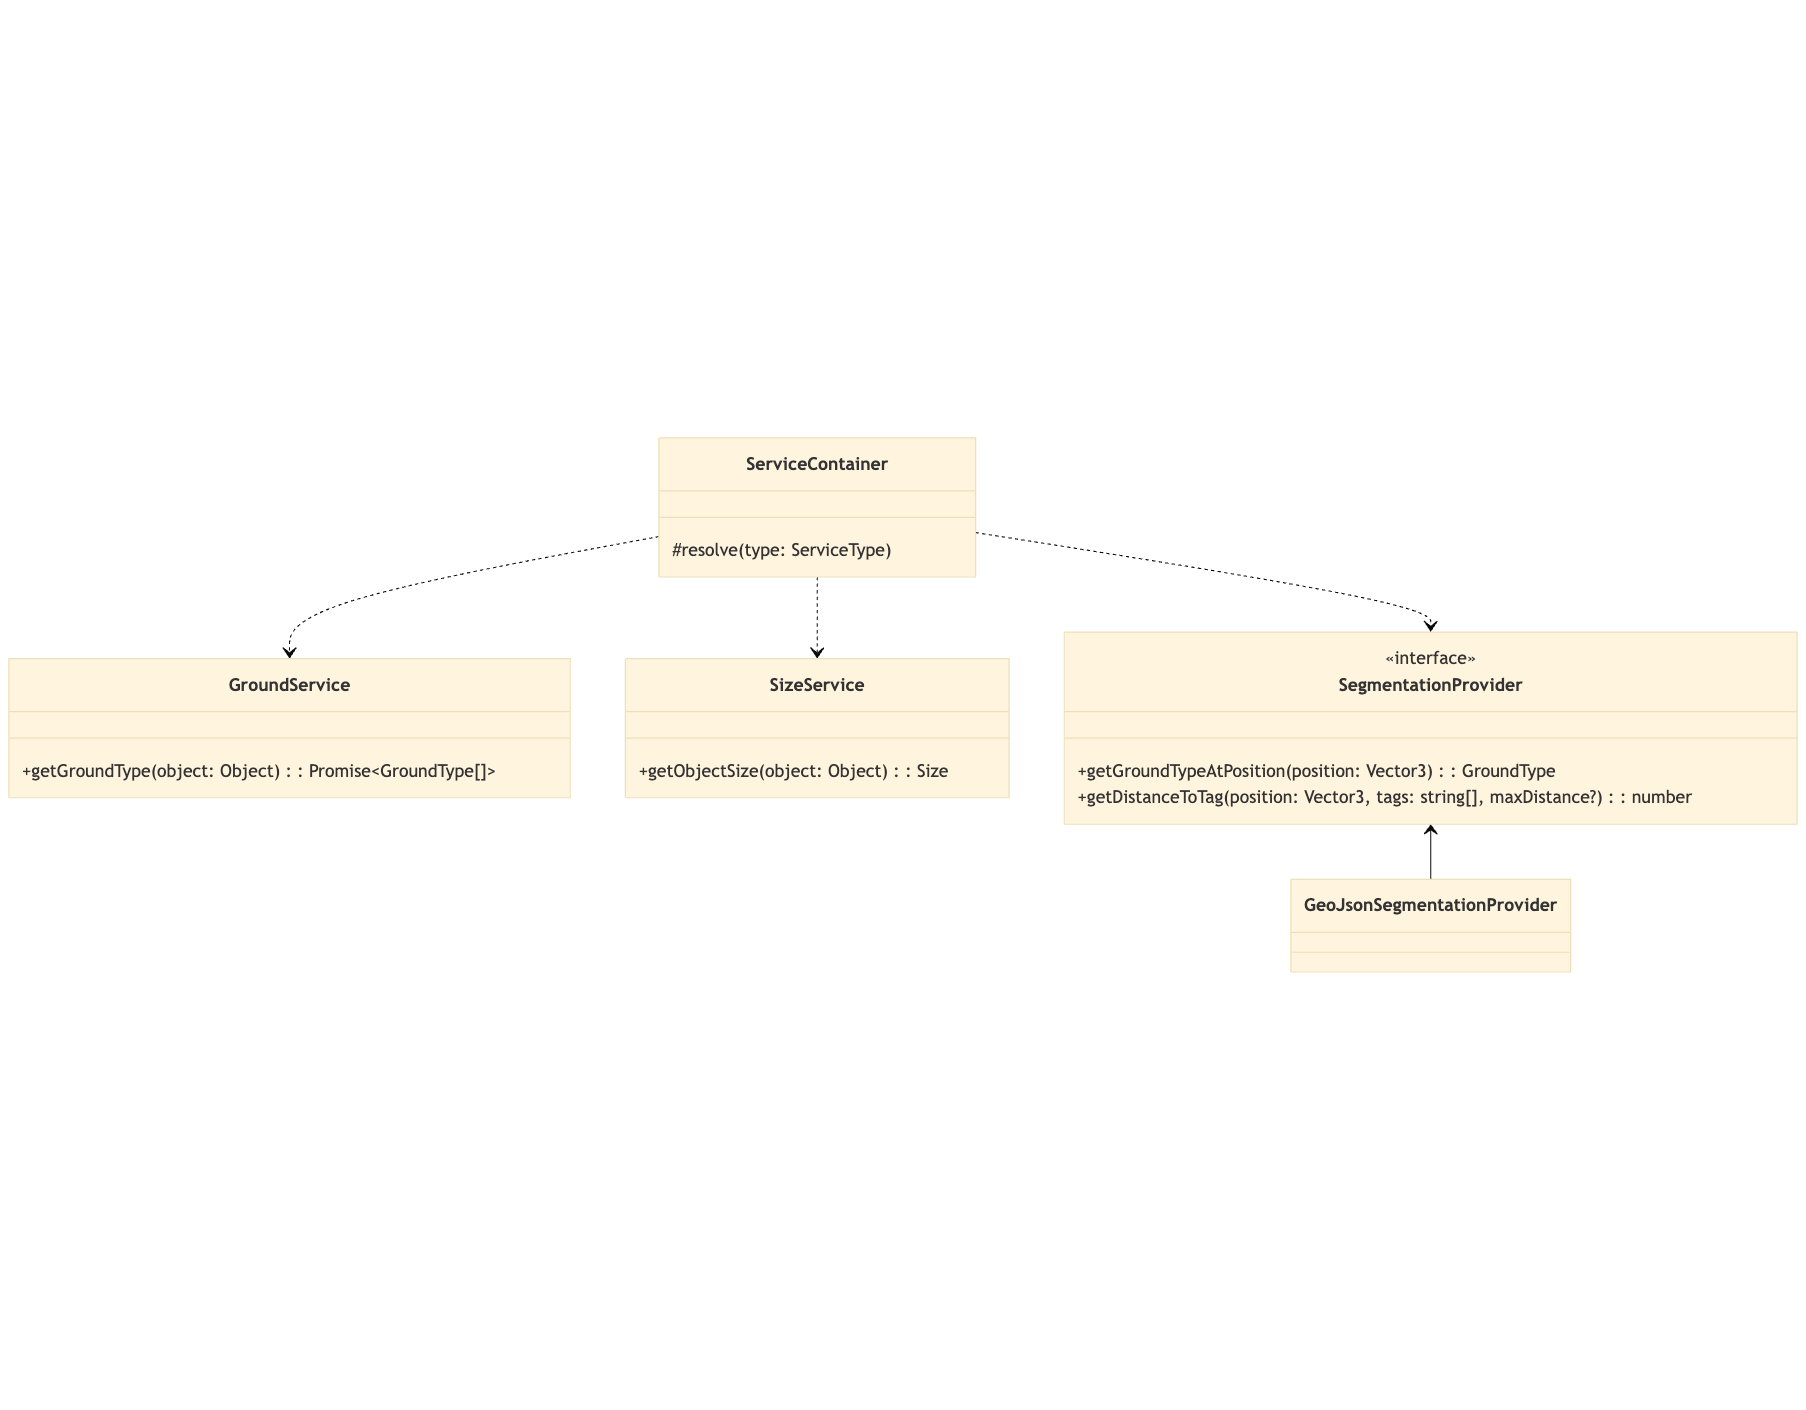
\includegraphics[width=1\textwidth]{abb/uml infrastructure.png}
\centering
\caption{Klassendiagramm: Infrastructure Layer}
\label{fig:uml infrastructure}
\end{figure}

Abbildung \ref{fig:uml infrastructure} zeigt ein UML Klassendiagramm des Aufbaus der Layers, wobei die einzelnen Services innerhalb der Validatoren mittels des IoC ServiceContainers aufgelöst werden.

Der \textmono{GroundService} stellt die Methode \textmono{getGroundType} zur Bestimmung, welche Untergrundarten sich unter einem Objekt befindet. Intern prüft diese Funktion, welcher Untergrund sich an den vier äußersten Ecken des Objekts befindet. Zur Berechnung der Ecken nutzt der Service daher den \textmono{SizeService}.

Der \textmono{SizeService} stellt die Methode \textmono{getObjectSize} zur Berechnung der Eckpunkte eines Objekts anhand der Objektmodels, der eingestellten Größe, Position und Rotation. Aufgrund der Abhängigkeit des konkreten Objektmodels lädt und cached diese Klasse intern die Objektmodelle im Gltf-Format.

Der \textmono{SegmentationProvider} stellt schließlich eine Möglichkeit, auf die Segmentierungsinformationen an bestimmten Punkten des 3D-Raums zuzugreifen. Da die Segmentierung 

\subsubsection{AR-Basissystem: Presentation Layer}

// EffectableGltf

\subsection{Testing}

\subsection{Virtuelle Straßenumgebung}

\subsection{Performance-Messung}

